\part{Introduction of the Green FabLab}

\chapter{Context of the project}

\section{Presentation of the project}

Since few years ago, the ERPI laboratory have been taking in place a research platform about innovation processes called the \textit{Lorraine Fab Living Lab} (LF2L).
This space joint a \textbf{«living lab»}, laboratory about the \textit{User Centered Design} concept, with a space \textbf{«FabLab»} that allows users in an easy and quick way to fabricate intermediary  objects in order to foster co-operation in engineering design \parencite{Boujut2003}.
Taking into account the notions of \textit{sustainability}, which is a currently  major societal issue, the \textit{FabLab} concept goes towards a notion of \textit{\textbf{Green FabLab}} with the purpose to better use  the resources present in these spaces.
This means to validate the concept of \textbf{local and distributed recycling process} thanks to the use of these innovation spaces (fablabs) and the 3D printing technology.

Figure \ref{Context} presents a global chain with main elements to consider in order to validate the concept.
In this context, various works have been and continue to be carried out, both from a technical  and logistical point of view.


\begin{figure}[H]
	\centering
	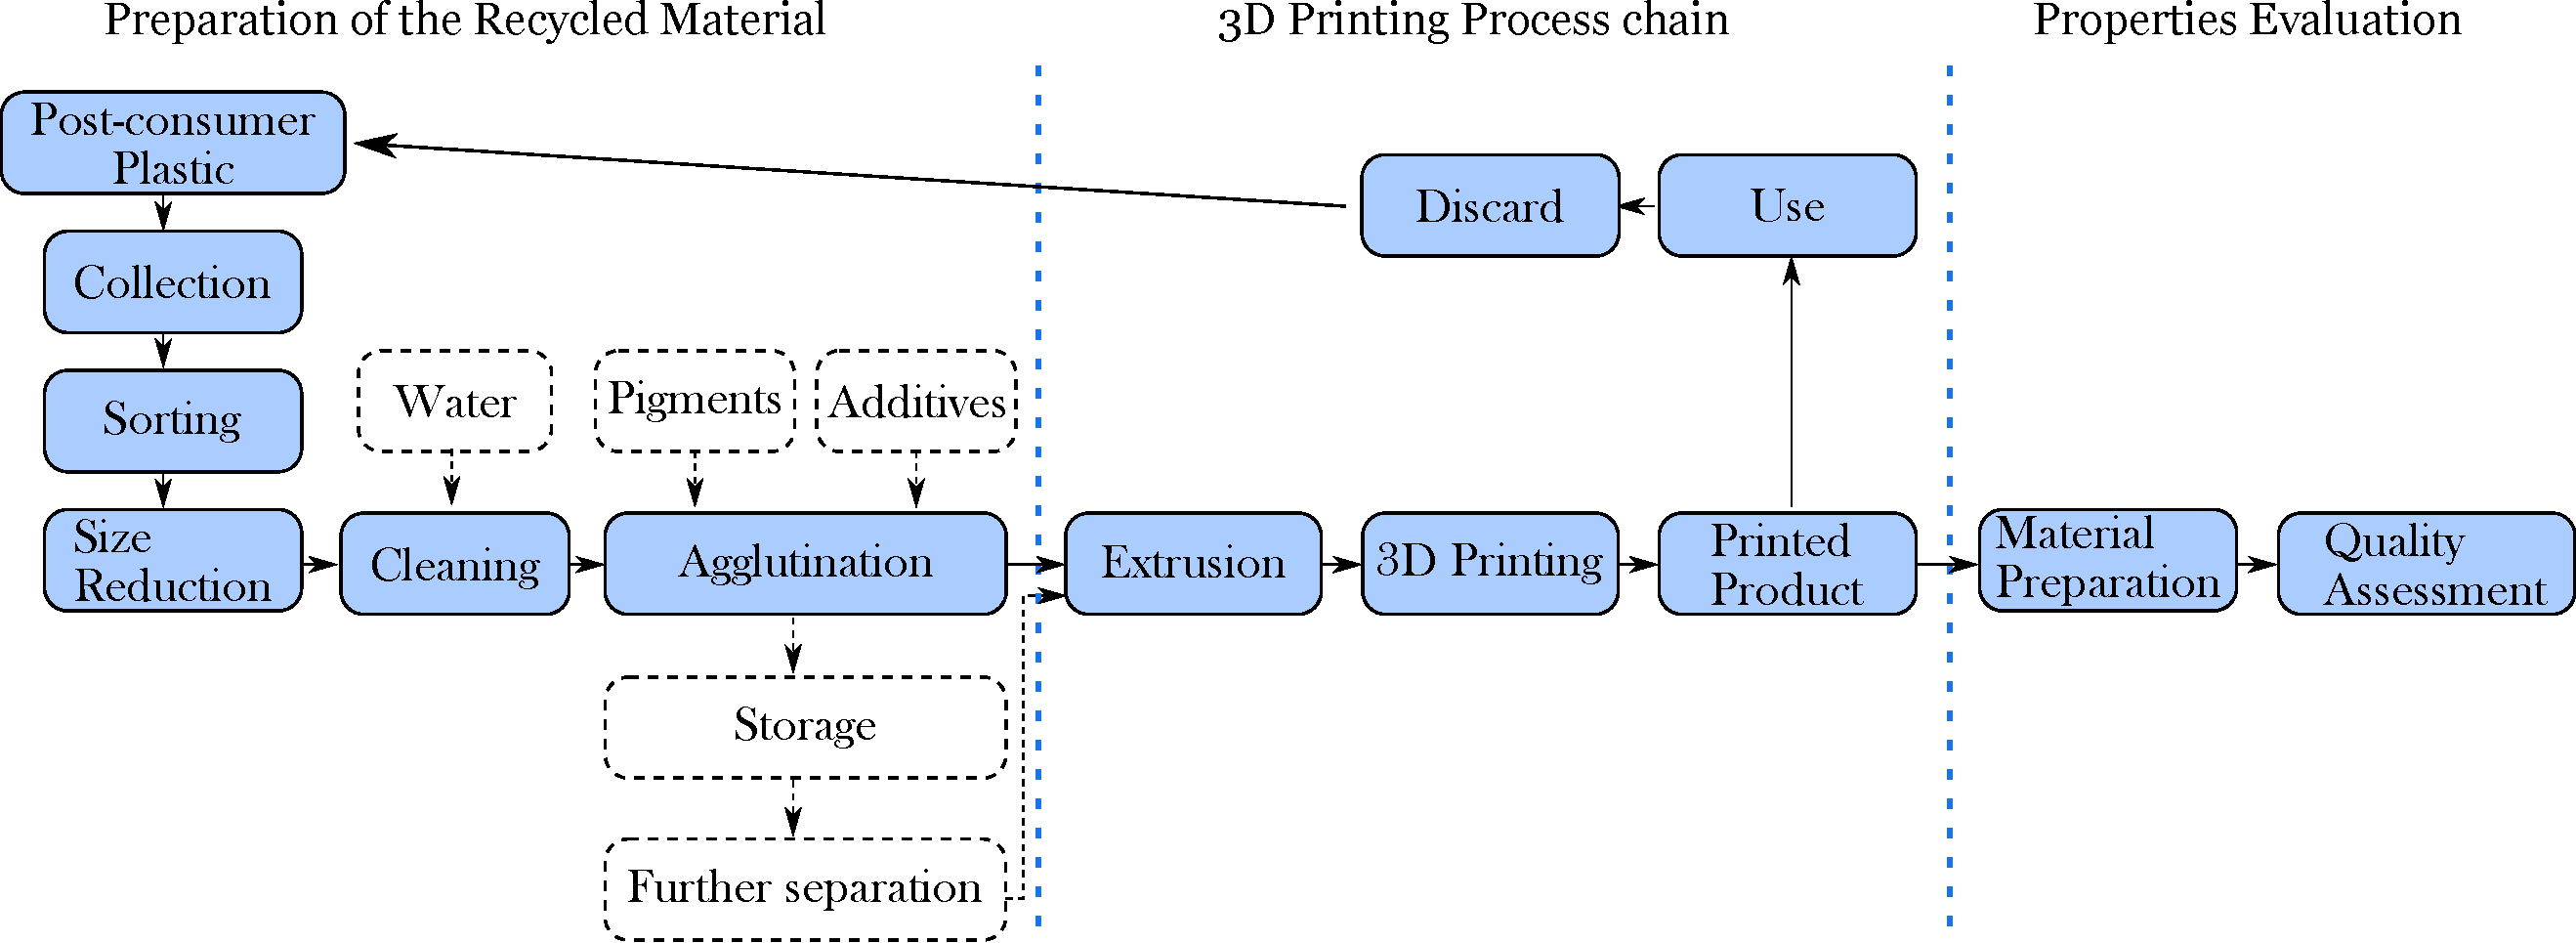
\includegraphics[width=\textwidth]{Figures/Mechanical-Recycling.pdf}
	\caption{Recycling process chain for opens-source additive manufacturing}
	\label{Context}
\end{figure}


In these context, we can differentiate three main dimensions:

\begin{description}
	\item[Technical :] Feasibility study of the process and the characteristics of the recycled materials.
	\item[Logistical :]  Characterization of the network needed in order to obtain raw materials   for local recycling.
	\item[Usage :] Define the notion of acceptability of the use for recycled material products
\end{description}


In the next section we describe in detail the three main aspect to study.

\section{Technical Aspect}

Figure \ref{3D.Printing.Chain} shows the technical elements in the 3D printing chain:

\begin{figure}[H]
	\centering
	\begin{tikzpicture}
	%\node[above, anchor=west, yshift=1.5cm, xshift=0.5cm] at (current page.west) {\alert{Only prototyping}};	
	\node[anchor=center, yshift=0cm, xshift=0.5cm, opacity=1, at=(current page.center)] {
		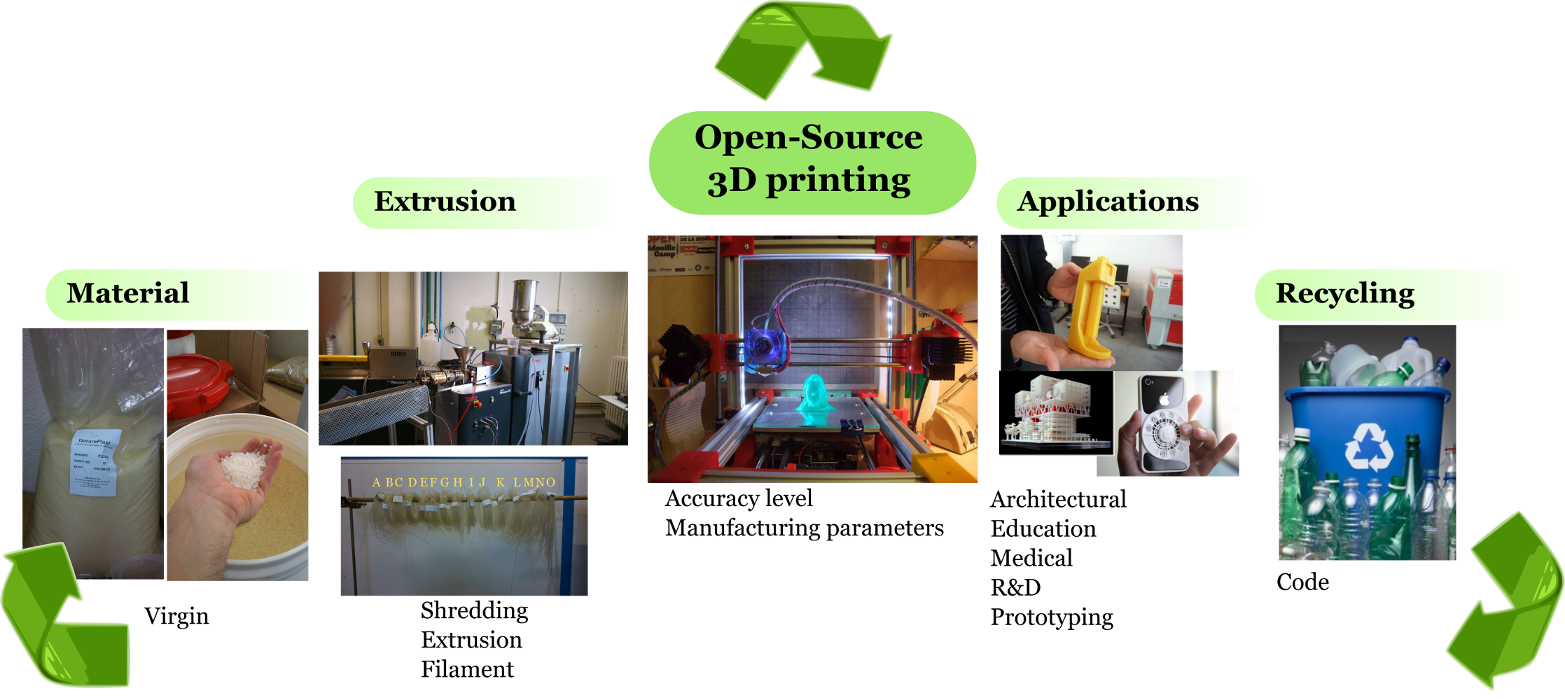
\includegraphics[width=0.8\textwidth]{Figures/General-Context-3DP-Recycling.png} };	
	\end{tikzpicture}
	\caption{Recycling process chain for opens-source Additive Manufacturing}
	\label{3D.Printing.Chain}
\end{figure}

The research project made by \textcite{CruzSanchez2017, CruzSanchez2014, Cruz2012}, in collaboration with the LRGP laboratory,  propose a methodology and a systematic process for polymer recycling with the purpose to reuse thermoplastic material into open-source 3D printers in te context of FabLabs; as illustrated in figure \ref{Recycling.3DP}.


\begin{figure}[H]
	\centering
	
	\begin{subfigure}{0.55\textwidth}
		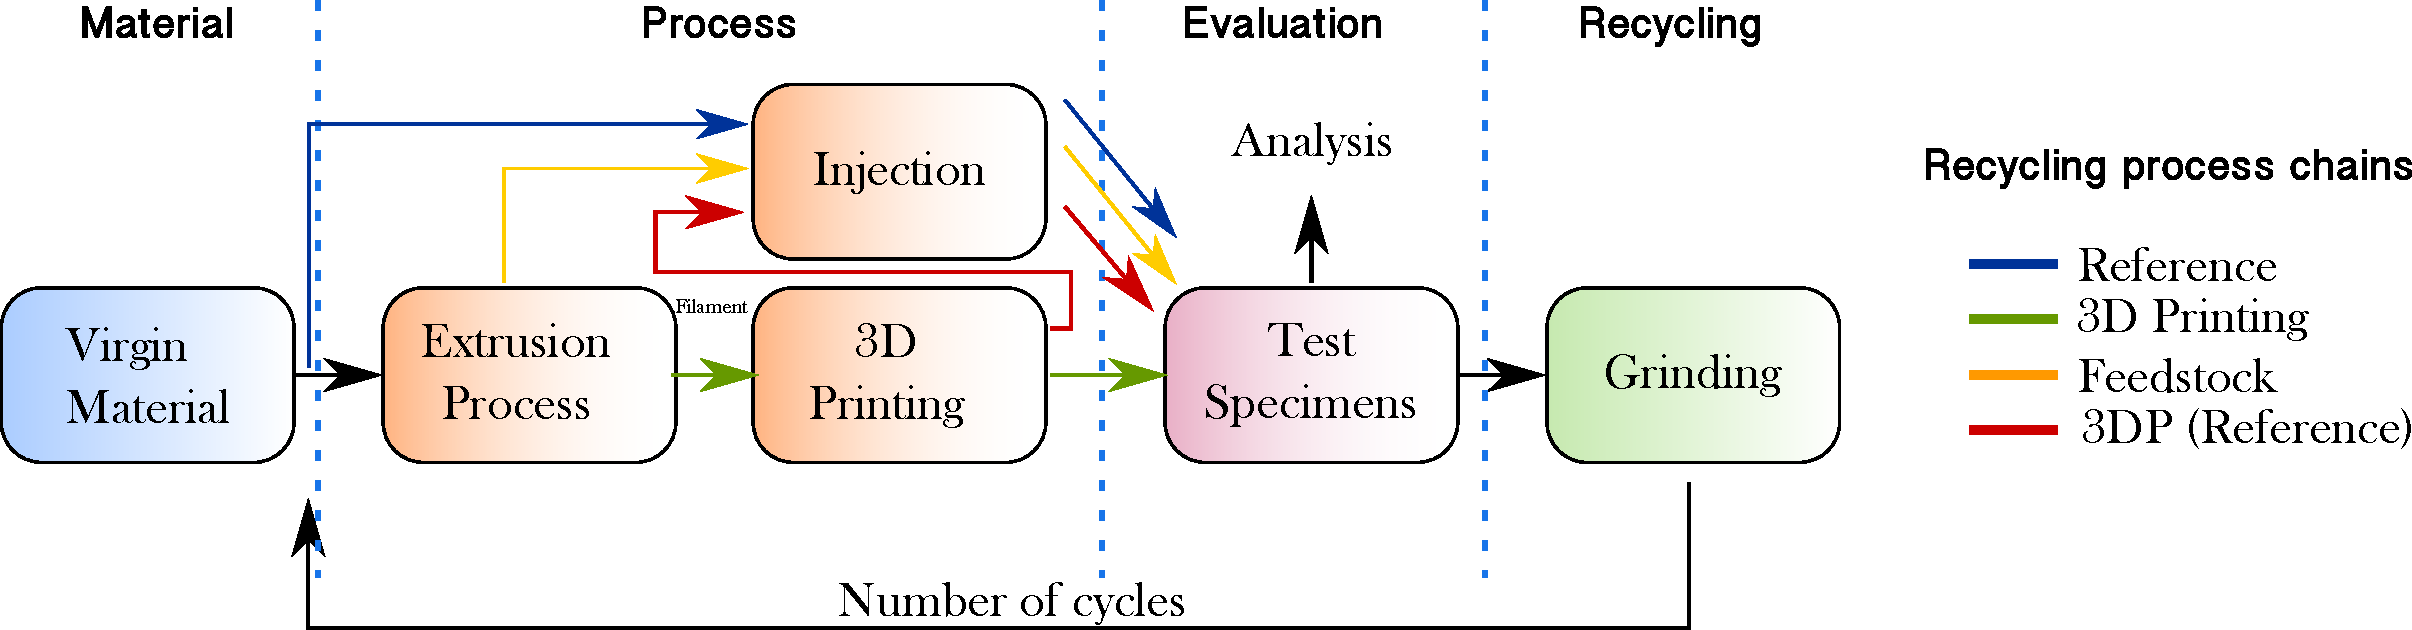
\includegraphics[width=\textwidth]{Figures/Recycling-framework.pdf}
		\caption{Methodological framework for recycling in 3DP.}
		\label{Recycling.Framework}
	\end{subfigure}
	\hfill
	\begin{subfigure}{0.4\textwidth}
		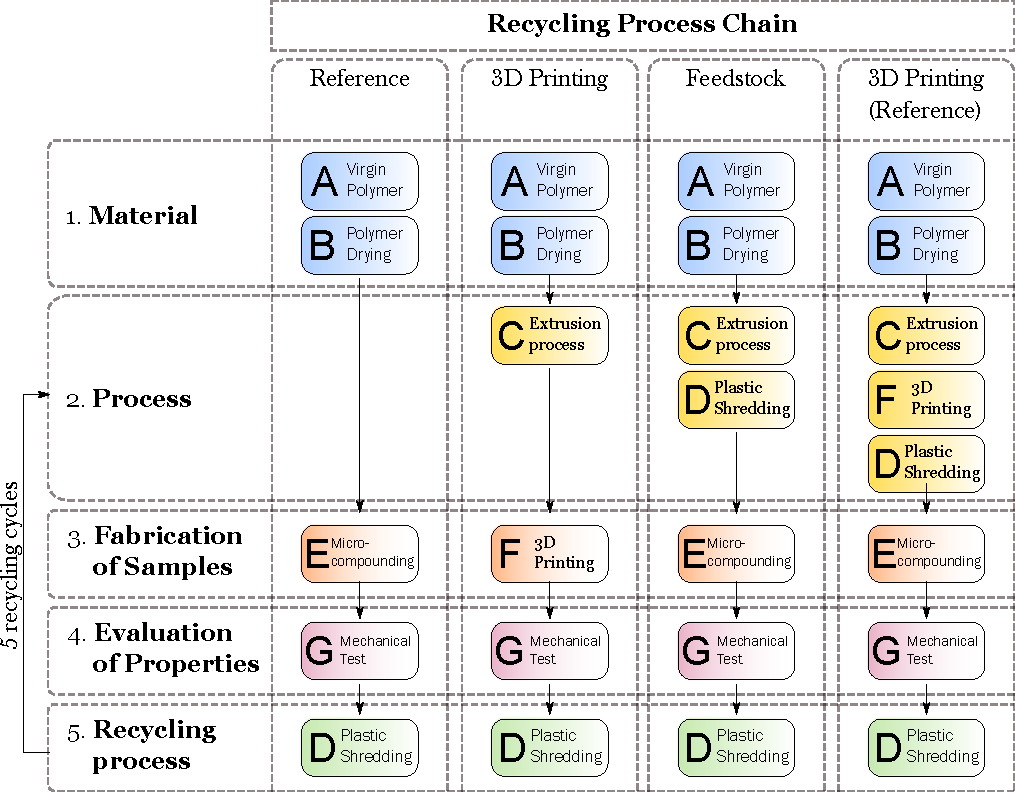
\includegraphics[width=\textwidth]{Figures/Operational-Methodology.pdf} 
		\caption{Operational methodology for recycling in 3DP.}
		\label{Operational.Methodology}		
	\end{subfigure}

		\label{Recycling.3DP}
\end{figure}

The main limits of this work are:

\begin{enumerate}
	\item Virgin material was considered as starting point of the recycling process.
	\item Only polylactic acid (PLA) was tested.
	\item Different processes such as \textit{sorting, cleaning, additives, pigments} were not considered in the recycling process.
	\item Laboratory conditions were used in the process. The fablab conditions are different in terms of cost, accuracy, etc.
\end{enumerate}
